\section{Multi-Graph Additions}
An additional contribution this work offers is the expansion to night vs day charging. During the night, there is one charger for each bus; each with a single charge rate.  During this time, buses are also available to charge at any time.  These differences in operations introduce changes to the original graph formation and warrent a separate graph.  
\par Night graphs consider a situation where both the number of buses reflecte the number of chargers and buses are readily available.  Note how there are several source and sink nodes in figure \ref{fig:nightVsDayGraph}.  When a bus deploys for the day, the available number of charges changes and are reflected in the underlying source and sink constraints.
\begin{figure*}
	\centering
	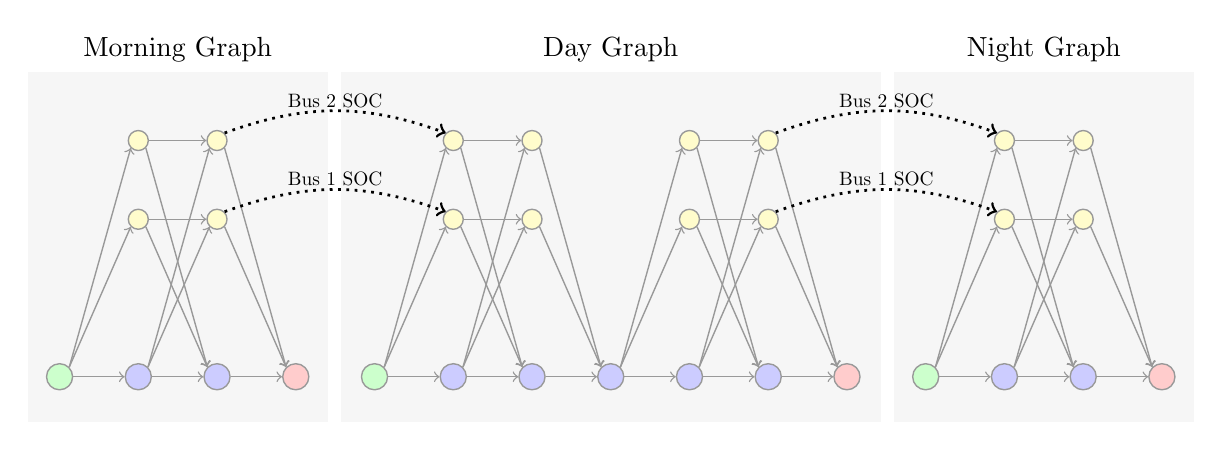
\begin{tikzpicture} 
		% morning graph
		\node[rectangle, fill=gray!7, minimum width=1.5in, minimum height=1.75in, label=above:Morning Graph](mBox) at (-2.5,1.65){};
		\node[circle, fill=green!20, line width=0.5pt, draw=black!40, minimum size=0.1in](mOne) at (-4,0){};
		\node[circle, fill=blue!20, line width=0.5pt, draw=black!40, minimum size=0.1in](mTwo) at (-3,0){}; 
		\node[circle, fill=blue!20, line width=0.5pt, draw=black!40, minimum size=0.1in](mThree) at (-2,0){};
		\node[circle, fill=red!20, line width=0.5pt, draw=black!40, minimum size=0.1in](mFour) at (-1,0){};

		\node[circle, fill=yellow!20, line width=0.5pt, draw=black!40, minimum size=0.1in, inner sep=1pt](mFive) at (-3,2){};
		\node[circle, fill=yellow!20, line width=0.5pt, draw=black!40, minimum size=0.1in, inner sep=1pt](mSix) at (-2,2){};
		\node[circle, fill=yellow!20, line width=0.5pt, draw=black!40, minimum size=0.1in, inner sep=1pt](mSeven) at (-3,3){};
		\node[circle, fill=yellow!20, line width=0.5pt, draw=black!40, minimum size=0.1in, inner sep=1pt](mEight) at (-2,3){};

		\draw[->, line width=0.5pt, color=black!40] (mOne.east) -- (mTwo.west){};
		\draw[->, line width=0.5pt, color=black!40] (mTwo.east) -- (mThree.west){};
		\draw[->, line width=0.5pt, color=black!40] (mThree.east) -- (mFour.west){};

		\draw[->, line width=0.5pt, color=black!40] (mOne.north east) -- (mFive.south west){};
		\draw[->, line width=0.5pt, color=black!40] (mTwo.north east) -- (mSix.south west){};
		\draw[->, line width=0.5pt, color=black!40] (mOne.north east) -- (mSeven.south west){};
                \draw[->, line width=0.5pt, color=black!40] (mTwo.north east) -- (mEight.south west){};

                \draw[->, line width=0.5pt, color=black!40] (mFive.south east) -- (mThree.north west){}; 
                \draw[->, line width=0.5pt, color=black!40] (mSix.south east) -- (mFour.north west){};
                \draw[->, line width=0.5pt, color=black!40] (mSeven.south east) -- (mThree.north west){};
		\draw[->, line width=0.5pt, color=black!40] (mEight.south east) -- (mFour.north west){};

                \draw[->, line width=0.5pt, color=black!40] (mFive.east) -- (mSix.west){};
                \draw[->, line width=0.5pt, color=black!40] (mSeven.east) -- (mEight.west){};

		% night graph
		\node[rectangle, fill=gray!7, minimum width=1.5in, minimum height=1.75in, label=above:Night Graph](nBox) at (8.5,1.65){};
		\node[circle, fill=green!20, line width=0.5pt, draw=black!40, minimum size=0.1in](nOne) at (7,0){};
		\node[circle, fill=blue!20, line width=0.5pt, draw=black!40, minimum size=0.1in](nTwo) at (8,0){}; 
		\node[circle, fill=blue!20, line width=0.5pt, draw=black!40, minimum size=0.1in](nThree) at (9,0){};
		\node[circle, fill=red!20, line width=0.5pt, draw=black!40, minimum size=0.1in](nFour) at (10,0){};

		\node[circle, fill=yellow!20, line width=0.5pt, draw=black!40, minimum size=0.1in, inner sep=1pt](nFive) at (8,2){};
		\node[circle, fill=yellow!20, line width=0.5pt, draw=black!40, minimum size=0.1in, inner sep=1pt](nSix) at (9,2){};
		\node[circle, fill=yellow!20, line width=0.5pt, draw=black!40, minimum size=0.1in, inner sep=1pt](nSeven) at (8,3){};
		\node[circle, fill=yellow!20, line width=0.5pt, draw=black!40, minimum size=0.1in, inner sep=1pt](nEight) at (9,3){};

		\draw[->, line width=0.5pt, color=black!40] (nOne.east) -- (nTwo.west){};
		\draw[->, line width=0.5pt, color=black!40] (nTwo.east) -- (nThree.west){};
		\draw[->, line width=0.5pt, color=black!40] (nThree.east) -- (nFour.west){};

		\draw[->, line width=0.5pt, color=black!40] (nOne.north east) -- (nFive.south west){};
		\draw[->, line width=0.5pt, color=black!40] (nTwo.north east) -- (nSix.south west){};
		\draw[->, line width=0.5pt, color=black!40] (nOne.north east) -- (nSeven.south west){};
                \draw[->, line width=0.5pt, color=black!40] (nTwo.north east) -- (nEight.south west){};

                \draw[->, line width=0.5pt, color=black!40] (nFive.south east) -- (nThree.north west){}; 
                \draw[->, line width=0.5pt, color=black!40] (nSix.south east) -- (nFour.north west){};
		\draw[->, line width=0.5pt, color=black!40] (nSeven.south east) -- (nThree.north west){};
		\draw[->, line width=0.5pt, color=black!40] (nEight.south east) -- (nFour.north west){};

		\draw[->, line width=0.5pt, color=black!40] (nFive.east) -- (nSix.west){};
                \draw[->, line width=0.5pt, color=black!40] (nSeven.east) -- (nEight.west){};


		% day graph	
		\node[rectangle, fill=gray!7, minimum width=2.7in, minimum height=1.75in, label=above:Day Graph](dBox) at (3,1.65){}; 
		\node[circle, fill=green!20, line width=0.5pt, draw=black!40, minimum size=0.1in](one) at (0,0){};
		\node[circle, fill=blue!20, line width=0.5pt, draw=black!40, minimum size=0.1in](two) at (1,0){}; 
		\node[circle, fill=blue!20, line width=0.5pt, draw=black!40, minimum size=0.1in](three) at (2,0){};
		\node[circle, fill=blue!20, line width=0.5pt, draw=black!40, minimum size=0.1in](four) at (3,0){};
		\node[circle, fill=blue!20, line width=0.5pt, draw=black!40, minimum size=0.1in](five) at (4,0){};
		\node[circle, fill=blue!20, line width=0.5pt, draw=black!40, minimum size=0.1in](six) at (5,0){};
		\node[circle, fill=red!20, line width=0.5pt, draw=black!40, minimum size=0.1in](seven) at (6,0){};
		
		\node[circle, fill=yellow!20, line width=0.5pt, draw=black!40, minimum size=0.1in, inner sep=1pt](eight) at (1,2){};
		\node[circle, fill=yellow!20, line width=0.5pt, draw=black!40, minimum size=0.1in, inner sep=1pt](nine) at (2,2){};
		\node[circle, fill=yellow!20, line width=0.5pt, draw=black!40, minimum size=0.1in, inner sep=1pt](ten) at (4,2){};
		\node[circle, fill=yellow!20, line width=0.5pt, draw=black!40, minimum size=0.1in, inner sep=1pt](eleven) at (5,2){};

		\node[circle, fill=yellow!20, line width=0.5pt, draw=black!40, minimum size=0.1in, inner sep=1pt](twelve) at (1,3){};
		\node[circle, fill=yellow!20, line width=0.5pt, draw=black!40, minimum size=0.1in, inner sep=1pt](thirteen) at (2,3){};
		\node[circle, fill=yellow!20, line width=0.5pt, draw=black!40, minimum size=0.1in, inner sep=1pt](fourteen) at (4,3){};
		\node[circle, fill=yellow!20, line width=0.5pt, draw=black!40, minimum size=0.1in, inner sep=1pt](fifteen) at (5,3){};

		\draw [->, line width=0.5pt, color=black!40] (one.east) -- (two.west);
		\draw [->, line width=0.5pt, color=black!40] (two.east) -- (three.west);
		\draw [->, line width=0.5pt, color=black!40] (three.east) -- (four.west);
		\draw [->, line width=0.5pt, color=black!40] (four.east) -- (five.west);
		\draw [->, line width=0.5pt, color=black!40] (five.east) -- (six.west);
		\draw [->, line width=0.5pt, color=black!40] (six.east) -- (seven.west);

		\draw [->, line width=0.5pt, color=black!40] (one.north east) -- (eight.south west);
		\draw [->, line width=0.5pt, color=black!40] (two.north east) -- (nine.south west);
		\draw [->, line width=0.5pt, color=black!40] (four.north east) -- (ten.south west);
		\draw [->, line width=0.5pt, color=black!40] (five.north east) -- (eleven.south west);
		\draw [->, line width=0.5pt, color=black!40] (eight.south east) -- (three.north west);
		\draw [->, line width=0.5pt, color=black!40] (nine.south east) -- (four.north west);
		\draw [->, line width=0.5pt, color=black!40] (ten.south east) -- (six.north west);
		\draw [->, line width=0.5pt, color=black!40] (eleven.south east) -- (seven.north west);
		\draw [->, line width=0.5pt, color=black!40] (eight.east) -- (nine.west);
		\draw [->, line width=0.5pt, color=black!40] (ten.east) -- (eleven.west); 

		\draw [->, line width=0.5pt, color=black!40] (one.north east) -- (twelve.south west);
		\draw [->, line width=0.5pt, color=black!40] (two.north east) -- (thirteen.south west);
		\draw [->, line width=0.5pt, color=black!40] (four.north east) -- (fourteen.south west);
		\draw [->, line width=0.5pt, color=black!40] (five.north east) -- (fifteen.south west);
		\draw [->, line width=0.5pt, color=black!40] (twelve.south east) -- (three.north west);
		\draw [->, line width=0.5pt, color=black!40] (thirteen.south east) -- (four.north west);
		\draw [->, line width=0.5pt, color=black!40] (fourteen.south east) -- (six.north west);
		\draw [->, line width=0.5pt, color=black!40] (fifteen.south east) -- (seven.north west);
		\draw [->, line width=0.5pt, color=black!40] (twelve.east) -- (thirteen.west);
		\draw [->, line width=0.5pt, color=black!40] (fourteen.east) -- (fifteen.west); 


		\draw [dotted, color=black,-,line width=1pt] (mSix.north east) edge[->,bend left=20pt]node[above=-2.5pt]{\scalebox{0.7}{Bus 1 SOC}}(eight.north west); 
		\draw [dotted, color=black,-,line width=1pt] (mEight.north east) edge[->,bend left=20pt]node[above=-2.5pt]{\scalebox{0.7}{Bus 2 SOC}}(twelve.north west);

		\draw [dotted, color=black,-,line width=1pt] (eleven.north east) edge[->,bend left=20pt]node[above=-2.5pt]{\scalebox{0.7}{Bus 1 SOC}}(nFive.north west); 
		\draw [dotted, color=black,-,line width=1pt] (fifteen.north east) edge[->,bend left=20pt]node[above=-2.5pt]{\scalebox{0.7}{Bus 2 SOC}}(nSeven.north west);
	\end{tikzpicture}
	\caption{Night vs Day Graphs}
	\label{fig:nightVsDayGraph}
\end{figure*}
\par Changes in the first graph are reflected in the second through use of state of charge variables.
